\documentclass{beamer}
\usepackage[serbian]{babel}
\usetheme{Boadilla}
\usecolortheme{seahorse}
\usefonttheme{serif}

\usepackage{lipsum}
\usepackage{graphicx,xcolor}
\usepackage{amsmath,amssymb,amsfonts}

%\AtBeginSection[]{ 
    %\begin{frame}{Outline} 
   %     \tableofcontents[currentsection] 
 %   \end{frame} }

\title{Robotika u 2022.}
\subtitle{}
\institute[Tehničko i naučno pisanje]{Matematički fakultet\\Univerziteta u Beogradu}
\author[]{Đuro Cerović\\Marko Cvijetinović\\Luka Matić\\Mihajlo Radojević}
\date{12/2022}
%\titlegraphic{
\includegraphics[width=2cm]{images/logo/iiserm_logo.jpg}}

\begin{document}

\begin{frame}
\titlepage
\end{frame}


\section{Uvod}
%\input{segments/1_intro}
\begin{frame}{Uvod}
    \begin{itemize}
        \item Uticaj ubrzanog razvoja nauke i tehnike na industriju i društvo
        \item Ulaganje u razvoj novih tehnologija  od kojih je jedna robotika
        \item Robotika je nova nauka koja obuhvata više naučnih polja
        \item Robot kao zamena za ljudski napor
        \item Asimovljevi zakoni robotike
    \end{itemize}
    \begin{figure}
        \centering
        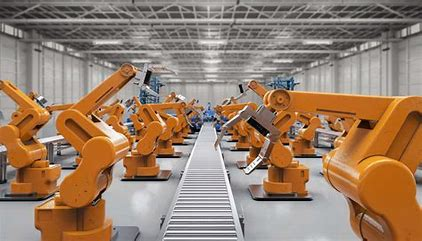
\includegraphics[scale=0.45]{roboti.png}   
    \end{figure}
\end{frame}
 
\section{Saradnički roboti}
\begin{frame}{Saradnički roboti}
    \begin{itemize}
        \item Rast potražnje zbog pandemije
        \item Preuzimaju suvoparne, prljave i opasne poslove
        \item Automatizacija procesa dovodi do veće preciznosti i efikasnosti 
        \item Imaju veliku primenu u fabrikama 
    \end{itemize}
    \begin{figure}
        \centering
        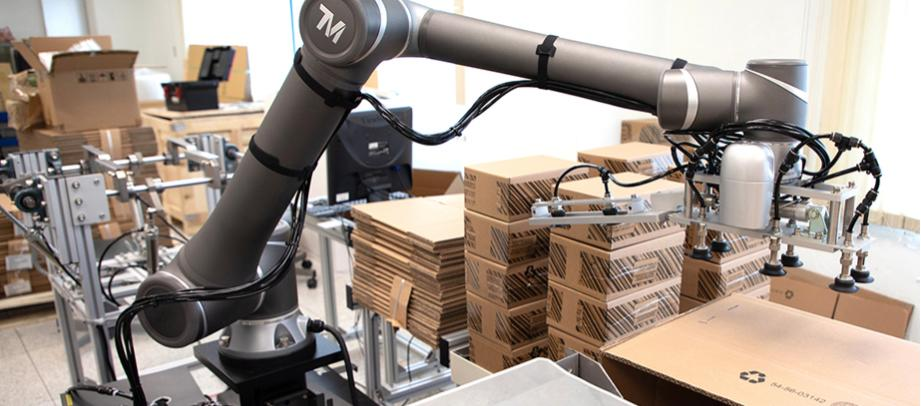
\includegraphics[scale=0.25]{Cobot.jpg}
    \end{figure}
\end{frame}

\section{Roboti dostavljači}
\begin{frame}{Roboti dostavljači}
    \begin{itemize}
        \item Nastali radi smanjenja kontakta izmedju ljudi
        \item Fleksibilniji od ljudi jer mogu da rade 24/7
        \item Povećanje potražnje za brzom dostavom doprinosi njihovoj popularnosti
    \end{itemize}
    \begin{figure}
        \centering
        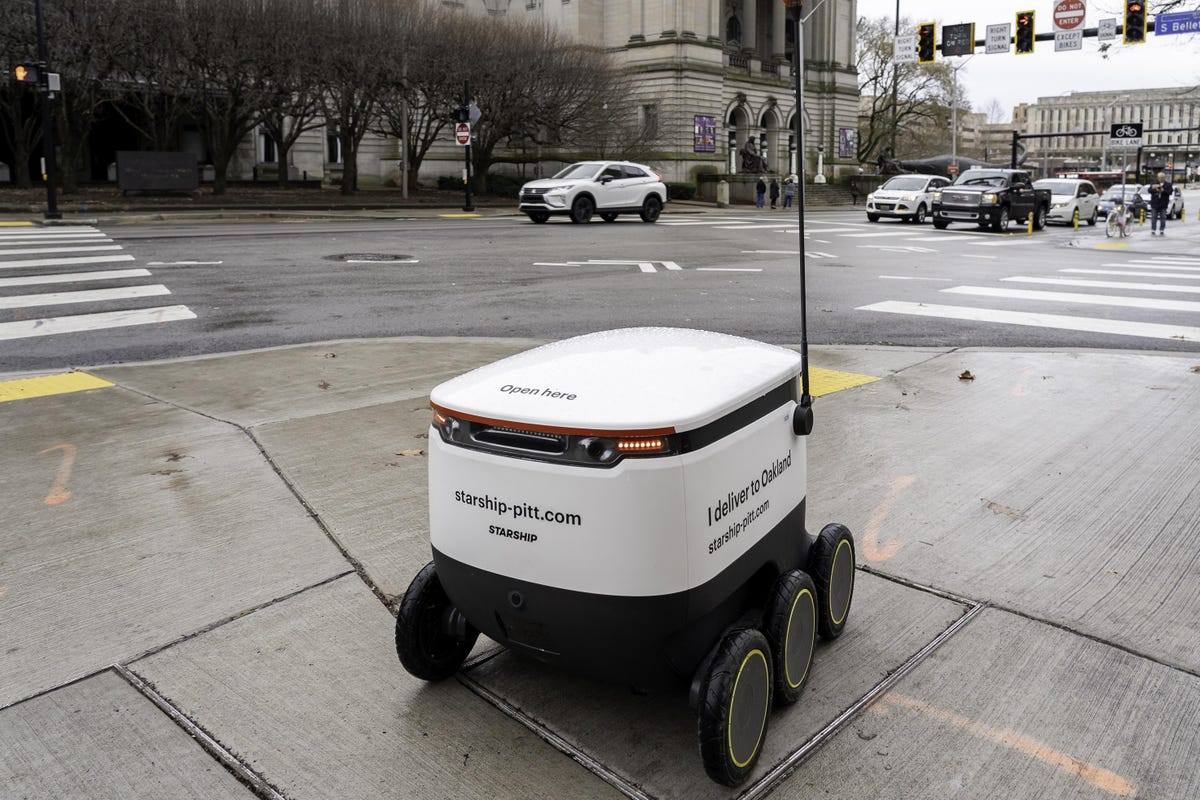
\includegraphics[scale=0.15]{DeliveryRobot.jpg}
    \end{figure}
\end{frame}

\section{Conclusion}
%\input{segments/4_conclude}


\section*{References}
\begin{frame}
    \frametitle{References}
    \bibliographystyle{amsalpha}
    \bibliography{ref.bib}
\end{frame}

\end{document}